\chapter{Algorithm}
\label{chapter:algorithm}

In this chapter we describe the algorithm used by ACE. We give a general
overview over the concepts. However, the interested reader is referred to
the documentation of the semester project for a detailed description (see 
\emph{Report Evaluation Algorithm}). This chapter is only intended to give
the reader enough information to understand the basic concepts and the
design decisions made in the implementation.



\section{Introduction}
Real-time cooperative editing systems allow multiple users to view and edit the 
same document at the same. The changes of other participants in an editing
session are immediately visible on the local screen. Consistency maintenance
is one of the most significant challenges in designing and implementing
these systems. Fortunately, researchers have found algorithms that solve the
problems present in these systems.


\subsection{Requirements}
The following requirements have been identified for synchronous collaborative
editing systems.

\subsubsection{Real-time} 
The response to local user actions must be quick, ideally
as quick as a single-user editor. Imposing a global total order is not
an option because of the distributed nature of the system (i.e. network
latency). Thus, generally these systems replicate the document at each
user's site.

\subsubsection{Distributed} 
Cooperating users reside on different machines 
connected by communication networks with nondeterministic latency.

\subsubsection{Unconstrained} 
Multiple users are allowed to concurrently and
independently edit any part of the document at any time, in order to 
facilitate free and natural information flow among multiple users.


\subsection{Document Model}
In the following we assume a (conceptual) shared document model that consists 
of a sequence of characters, indexed from 0 up to the number of characters in
the document minus 1. The document state (i.e. the text) can only be 
modified by executing one of the following two primitive editing operations:

\begin{itemize}
 \item Insert(p, str): insert the String $str$ at position $p$
 \item Delete(p, len): delete $len$ characters starting at position $p$
\end{itemize}

Each participant in an editing session has a replica of the document, to which
he/she applies the changes.


\subsection{Preliminaries}
In this section, some basic concepts and terminologies are introduced. Following Lamport~\cite{lamport78}, we define a causal (partial) ordering relation on operations in terms of their generation and execution sequences as follows.

\begin{defn}
Causal ordering relation $\rightarrow$
\end{defn}

Given two operations $O_{a}$ and $O_{b}$ generated at sites $i$ and $j$, then $O_{a}\rightarrow O_{b}$, iff:
\begin{enumerate}
 \item $i=j$ and the generation of $O_{a}$ happened before the generation of 
       $O_{b}$
 \item or $i \neq j$ and the execution of $O_{a}$ at site $j$ happened before 
       the generation of $O_{b}$
 \item or there exists an operation $O_{x}$ such that $O_{a}\rightarrow O_{x}$
       and $O_{x}\rightarrow O_{b}$
\end{enumerate}

Note that the causal ordering relation is a \emph{partial ordering}.

\begin{defn}
Dependent and independent operations
\end{defn}

Given any two operations $O_{a}$ and $O_{b}$:
\begin{enumerate}
 \item $O_{b}$ is \emph{dependent} on $O_{a}$ iff $O_{a} \rightarrow O_{b}$
 \item $O_{a}$ and $O_{b}$ are \emph{independent} (or \emph{concurrent}), 
       expressed as $O_{a} \Arrowvert O_{b}$ iff neither 
       $O_{a}\rightarrow O_{b}$ nor $O_{b}\rightarrow O_{a}$
\end{enumerate}

Intuitively we can say that two operations are dependant if there exists a path from the generation of one message to the generation of another message. So for example in figure \ref{fig:example1} operation $O_{1}$ and $O_{3}$ are dependent, that is $O_{1}\rightarrow O_{3}$. Operation $O_{1}$ and $O_{2}$ are \emph{independent}. 

\begin{figure}
 \centering
 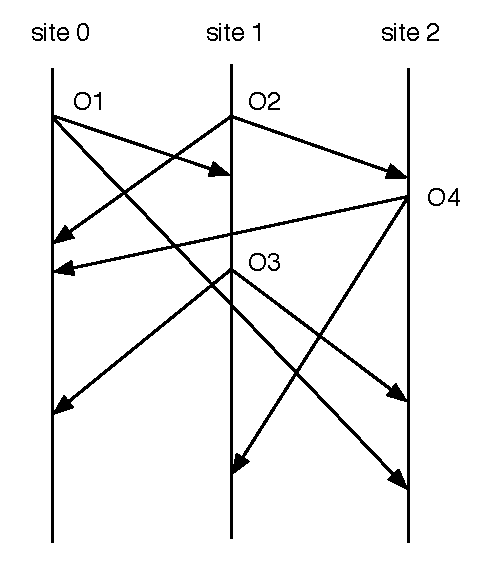
\includegraphics[width=2.5in,height=2.88in]{../images/finalreport/example1.eps}
 \caption{A scenarion of a real-time cooperative editing session}
 \label{fig:example1}
\end{figure}

\subsubsection{Vector Time}
Most algorithms, including the one we implemented,
use \emph{vector times} to determine the causal ordering relation. Each site
maintains a state vector $v$ that has $n$ components where $n$ is the number of 
participating sites. $S$ is the local site. The $i$-th component of $v$ denoted 
as $v[i]$ represents the number of operations executed from site $i$ at site 
$S$. 

\begin{defn}
  For two time vectors u, v \\
  $u \leq v$ iff $\forall i : u[i] \leq v[i]$ \\
  $u < v$ iff $u \leq v$ and $u \not= v$ \\
  $u \parallel v$ iff $\neg(u < v)$ and $\neg(v < u)$
\end{defn}

Notice that $\leq$ and $<$ are partial orders. The \emph{concurrency relation} 
$\parallel$ is reflexive and symmetric.

The above definition gives us a very simple method to decide whether two events 
$e$ and $e'$ are causally related or not: We take their timestamps (vector 
times) and check whether $C(e) < C(e')$ or $C(e') < C(e)$ where $C(x)$ 
determines the timestamp of $x$. If the test succeeds, the events are causally 
related. Otherwise they are independent.


\subsection{Consistency Model}
A cooperative editing system is said to be consistent if it always maintains the
following properties:

\subsubsection{Convergence} 
When the system is at quiescence (i.e. no messages are
in transit), all copies of the shared document are identical.

\subsubsection{Causality-Preservation} 
For any pair of operations $O_a$ and $O_b$,
if $O_a \rightarrow O_b$ then $O_a$ is executed before $O_b$ at all sites.

\subsubsection{Intention-Preservation} 
For any operation $O$, the effects of
executing $O$ at all sites are the same as the intention of $O$, and the effect
of executing $O$ does not change the effects of independent operations.


\subsection{Operational Transformation}
{Ellis and Gibbs}~\cite{ellis} proposed a new concept for
consistency control, called \emph{Operational Transformation} (OT). 
Algorithms based on OT transform operations to include/exclude the effects of other operations. 
Intuitively, transformation shifts the position parameter of an
operation before execution to include/exclude the effects of previously executed
operations that it was not \emph{aware} of (or that are concurrent) at the
time of its generation. Operation transformation also helps to solve the
problem of intention violation.

An operational transformation algorithm is typically split into two parts. 
First, an application independent consistency control algorithm which determines 
what operations need to be transformed against what other operations. Second,
a set of application dependent transformation functions. There are two
types of transformation functions, inclusion transformation (IT) and 
exclusion transformation (ET). All operational transformation algorithms
use inclusion transformation, whereas exclusion transformation is used
by fewer OT algorithms.

A transformation function has to be defined for every combination of operations.
So for a text editor with the two primitive operations \emph{insert} and
\emph{delete} as defined above, there would be a total of four transformation
functions for IT and another four for ET. That is, given a transformation
function T the following four transformation functions have to be defined:
T(\emph{insert,insert}), T(\emph{insert,delete}), T(\emph{delete,insert}), 
and T(\emph{delete,delete}).

\subsubsection{Inclusion Transformation}
Inclusion transformation includes the effect of another operation into an
operation. The precondition of IT is that both operations are defined on the
same document state (i.e. have the same vector time). If we have an operation
$O_1 = Ins(0,'a')$, an operation $O_2 = Del(1,1)$ (both defined on the same
document state) and the document state \emph{123}, we can either first
execute $O_1$ or $O_2$. If we execute $O_1$ first, we cannot execute $O_2$
as it is. That is where IT comes into play:

$$ IT(O_1,O_2) = O'_2 = Del(2,1) $$

The transformed operation can be applied to the document resulting in the
correct document state \emph{b13}.

\subsubsection{Exclusion Transformation}
Exclusion transformation transforms an operation $O_1$ against another operation
$O_2$ in such a way that the impact of $O_2$ is effectively excluded from
$O_1$. As exclusion transformation is not used by the selected algorithm, we
refer the interested reader to the \emph{Report Evaluation Algorithm} for
a more complete definition of exclusion transformation.


\subsection{Transformation Properties}
Depending on the used operational transformation algorithm, the transformation
functions must satisfy certain properties. The algorithm used by ACE must
only satisfy the so called transformation property 1 (TP1). 

\paragraph{Transformation Property 1:}
The transformation property 1 ensures that the effect of executing $O_1$
followed by the transformed request $O'_2$ is the same as executing
request $O_2$ followed by the transformed request $O'_1$.

\begin{defn}
Transformation Property 1 (TP1):
$ O_1 O'_2 \equiv O_2 O'_1 $
\end{defn}



\section{Selection of Algorithm}
In the semester project we made an extensive evaluation of existing algorithms
(see \emph{Report Evaluation Algorithm}). Based on the following selection
criteria we selected on algorithm.


\subsection{Selection Criteria}

\subsubsection{Correctness} 
Some algorithms proved to be incorrect in certain
cases. This is of course the most important selection criteria.

\subsubsection{Availability of Information} 
Some papers did not provide enough
information for an implementation of the described algorithm.

\subsubsection{Availability of User Undo} 
Users of collaborative applications
expect the same commands as in a single user application. 

\subsubsection{Algorithmic Complexity} 
Some algorithms are strikingly simple,
others are complex, and some are even too complex to be implemented.


\subsection{Selection of Algorithm}
The two only algorithms that satisfied the above criteria were 
\emph{adOPTed}~\cite{ressel96} and \emph{Jupiter}~\cite{jupiter95}. The 
following list shows why we have decided to implement \emph{Jupiter}:

\begin{itemize}
 \item \emph{Jupiter} is less complex than \emph{adOPTed}. The implementation of  \emph{adOPTed} contains a higher risk of unforeseen problems. 
 \item More technical issues remained unanswered on the \emph{adOPTed} 
algorithm, e.g. concurrent joining/writing. Therefore, we would have taken a 
higher risk when choosing \emph{adOPTed}.
 \item \emph{Jupiter} is more scalable. The number of 
communication paths in \emph{adOPTed} increases with $n(n-1)$, where $n$ is the 
number of clients. It only rises linearly with the number of clients in 
\emph{Jupiter}.
 \item The client/server model of \emph{Jupiter} better matches the spirit of collaborative editing, i.e. one client announces a document and becomes the server, whereas other clients connect with the server and join the collaborative editing session.
\end{itemize}

\subsection{Selection of Transformation Functions}
The \emph{Jupiter} algorithm makes use of a set of transformation functions.
However, no such functions are proposed in the paper. Therefore, we had to 
choose a set of transformation functions which would meet the needs of 
\emph{Jupiter}. The following list identifies the three preconditions for the 
transformation functions:

\begin{itemize}
 \item only IT required
 \item TP1 must be satisfied
 \item should be extensible to stringwise transformations
\end{itemize}

These three requirements where only met by one set of transformation
functions. They are described in the paper about \emph{GOTO}~\cite{sun98a}.



\section{Jupiter}
The \emph{Jupiter} system is a collaboration system that supports shared 
documents, shared tools, and, optionally, live audio/video communication. It was 
developed by \emph{Xerox}. It is conceptually a collaborative windowing toolkit. 
The low-level communication facilities make use of operational transformation.

The operational transformation algorithm employed in the \emph{Jupiter} system is derived from \emph{dOPT}. A centralized architecture and thus the reduction to point-to-point connections makes the algorithm significantly simpler than other operational transformation algorithms. The basic \emph{Jupiter} algorithm is only suitable for two sites. However, it was shown in \cite{jupiter95} and in greater detail in \cite{netedit:thesis} how to use several point-to-point connections to build a tree-structured $n$-site algorithm (see figure \ref{fig:concepts.nway}).

\begin{figure}[htb]
 \centering
 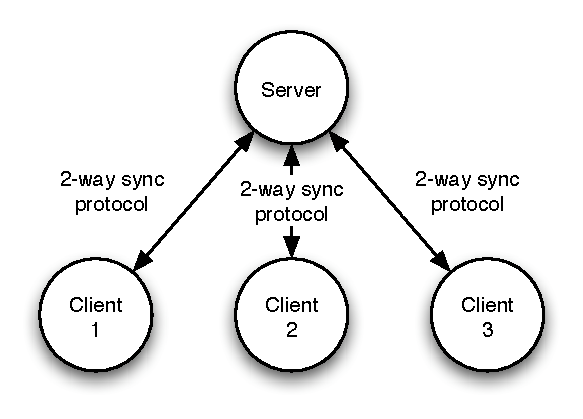
\includegraphics[width=7cm,height=4.89cm]{../images/finalreport/concepts_nway.eps}
 \caption{multiple 2-way sync to achieve n-way sync}
 \label{fig:concepts.nway}
\end{figure}

\subsection{Jupiter Algorithm}
A collaborative editing application requires that local operations are immediately applied to the local document and then sent inside a request to all
the other sites. Additionally to the operation, a request contains the vector
time of the sender. The vector time specifies the state the sender was in
(i.e. how many operations it has processed from itself and the receiver) just
before the new operation was generated.

Because the system does not impose a total ordering on the requests, it is
possible that two or more requests cross in transit. The general tool for 
handling these conflicting (i.e. concurrent) requests is a transformation function, called $xform$ in \cite{jupiter95}.

$$ xform(O_1,O_2)=\{O'_1,O'_2\} $$

This transformation function takes two operations, $O_1$ from the client and 
$O_2$ from the server, and returns two transformed operations $O'_1$ and $O'_2$.
The operations $O'_1$ and $O'_2$ have the property that if the client applies 
$O_1$ followed by $O'_2$, and the server applies $O_2$ followed by $O_1'$, both 
client and server wind up in the same final state (see figure 
\ref{fig:concepts.basic}). This property is also known as transformation property 1 (TP1):

$$ O_1 O'_2 \equiv O_2 O'_1 $$

Conceptually, the $xform$ function is a combined inclusion transformation (IT) 
that returns $\{IT(O_1,O_2),IT(O_2,O_1)\}$. The parameters $O_1$ and $O_2$ must 
originate from the same document state. This is a necessary precondition of 
inclusion transformation. If this precondition is violated, the result of the 
transformation is not guaranteed to be correct.

\begin{figure}[htb]
 \centering
 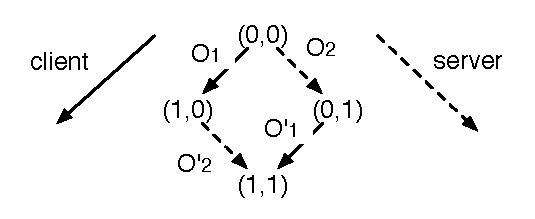
\includegraphics[width=6.85cm,height=2.5cm]{../images/finalreport/concepts_jupiter1.eps}
 \caption{basic transformation situation in jupiter}
 \label{fig:concepts.basic}
\end{figure}

\subsubsection{Point to Point}
As we have seen, it is helpful to show the two dimensional state space that both client and server pass through as they process requests (see figure \ref{fig:concepts.statespace}). Each state is labelled with the number of processed requests from both client and server to that point. For instance if the client is in the state $(2,3)$, it has generated and processed two requests of its own, and has received and processed three from the server. The client and server requests are displayed on different axis in the state space graph.

\begin{figure}[htb]
 \centering
 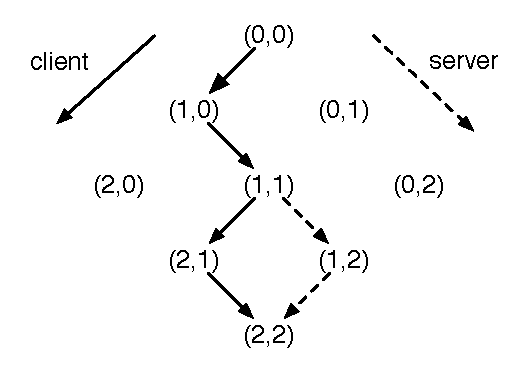
\includegraphics[width=6.63cm,height=4.5cm]{../images/finalreport/concepts_statespace.eps}
 \caption{two dimensional state space example}
 \label{fig:concepts.statespace}
\end{figure}

If there is a conflict, the paths will diverge, as shown in figure \ref{fig:concepts.statespace}. The client and server moved to the state $(1,1)$ together by first processing a client request, and then a server request. At that point, the client and server processed different requests (concurrently), moving to state $(2,1)$ and $(1,2)$ respectively. They each received and processed the other's message using the transformation function to move to state $(2,2)$.

As mentioned before, the algorithm labels each request with the state vector the
sender was in just before the message was generated (state vector). The 
recipient uses these state vectors to determine the causality relation.
If the request is not defined from the current state of the 
recipient, there is a conflict (concurrent request). Two concurrent requests 
have to be transformed, but they can only be transformed directly when they were 
generated from the same document state.

If client and server diverge by more than one step in the state space graph, the transformation function cannot be applied directly. Let us consider the state space in figure \ref{fig:concepts.statespace2}. The client has executed $c$ and receives the conflicting request $s_1$ from the server. It uses the transformation function to compute $s'_1$ to get to the state $(1,1)$. The server then generates $s_2$ from the state $(0,1)$, indicating that it still has not processed $c$. What should the client do now? It cannot use the transformation function directly because $c$ and $s_2$ were not generated from the same document state.

\begin{figure}[htb]
 \centering
 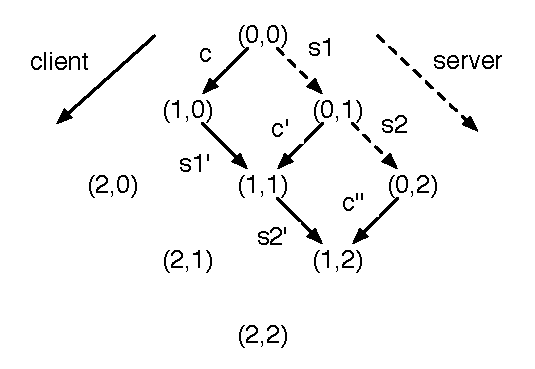
\includegraphics[width=6.71cm,height=4.5cm]{../images/finalreport/concepts_statespace2.eps}
 \caption{client and server diverging by more than one path step}
 \label{fig:concepts.statespace2}
\end{figure}

The solution to this situation is as follows. When the client computes $s'_1$ it 
must also remember $c'$. This represents a hypothetical request that the client 
could have generated to move from the state $(0,1)$ to $(1,1)$. When $s_2$
arrives, the client can use $c'$ to compute $c''$. It executes $s'_2$ to get to 
the state $(1,2)$. If the server has processed the client's message, it will be 
in the state $(1,2)$ as well. If not, its next request will originate from 
$(0,3)$, so the client saves $c''$ just in case.

The algorithm guarantees that if the transformation function satisfies TP1, then no matter how far the client and server diverge in state space, when they do reach the same state (and they do, unless requests get lost), they will have equivalent states (so convergence is achieved).

\subsubsection{Extending Jupiter to N-Way Communication}
We have discussed how a single two-way connection works in \emph{Jupiter}. We will now extend this systems to support $n$ clients using multiple two-way connections. The figure \ref{fig:concepts.nway-details} shows the basic setup for three clients. Each client talks only to the server over a standard previously discussed two-way connection. These standard two-way connections
are depicted in the figure. For each connection there are two algorithms:
$A_1$ and $A'_1$ for client 1, $A_2$ and $A'_2$ for client 2, and $A_3$ and
$A'_3$ for client 3.  

\begin{figure}[htb]
 \centering
 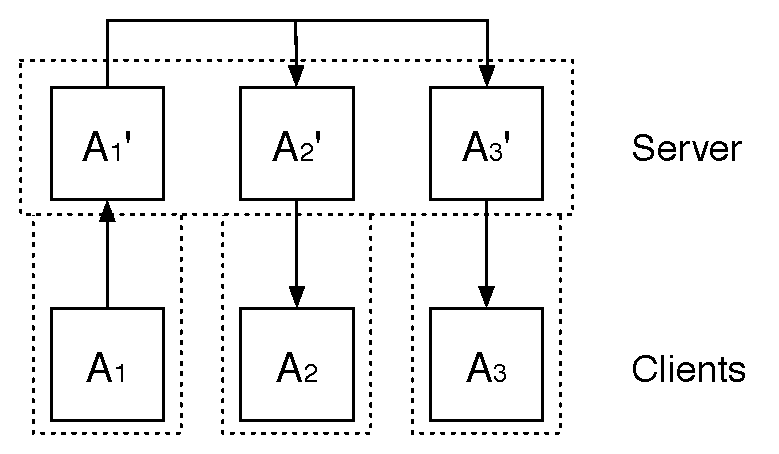
\includegraphics[width=6.31cm,height=3.56cm]{../images/finalreport/concepts_nway-details.eps}
 \caption{n-way synchronization using central server}
 \label{fig:concepts.nway-details}
\end{figure}

Let us say client 1 generates a local operation, for which the algorithm
creates a request. This request is sent to the server-side counterpart $A'_1$ of
this algorithm, which transforms the incoming request against any concurrent
requests (i.e. requests sent from the server that crossed that particular 
request in transit).

$A'_1$ extracts a (potentially) transformed operation from the received 
request. This operation is then given to the other server-side algorithms. 
In our example these are $A'_2$ and $A'_3$. These other algorithms create
requests for that operation and send these to $A_2$ and $A_3$ respectively.

\textbf{Note:} If \emph{Jupiter} is used in this setup, it is crucial that
only one request is processed at a time by the server. Processing of
requests from the clients must be serialized. Otherwise the setup cannot
guarantee consistency maintenance, most likely the replicas will diverge.

For an example how this setup works check the 
\emph{Report Implementation Algorithm}. There you find a simple example
of the n-way setup.


\subsection{Undo/Redo}
\label{sect:algorithm.undoredo}
% TODO: Undo/Redo
% 
% responsible: lukas zbinden
% describe why we could not implement undo/redo with Jupiter
%



\section{Implementation}


\subsection{Operation}
Operations are used to decribe changes made in a document. For this purpose they 
must contain the information what has been changed.

In case of simple text editing only two operations are required. An insert 
operation (e.g. \texttt{Ins(1,'hello')}) inserts the string 'hello' at position 
1 and an delete operation (e.g. \texttt{Del(10, 'world')}) deletes the string 
'world' at position 10.

\begin{figure}[H]
\centering
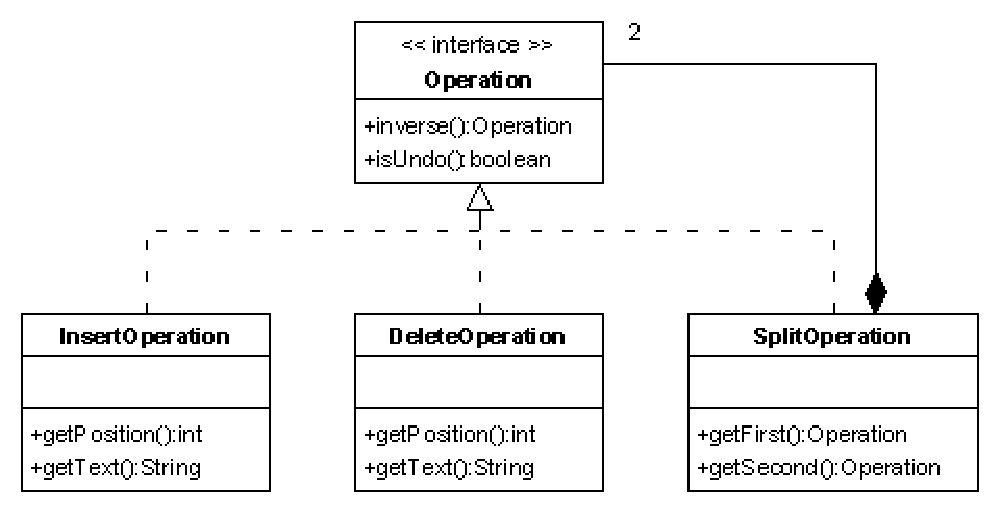
\includegraphics[height=5.74cm,width=11.59cm]{../images/finalreport/algorithm_operation.eps}
\caption{Operation Hierarchy}
\label{Operation Hierarchy}
\end{figure}

\label{Split_Operation}
As depicted in figure \ref{Operation Hierarchy} there exists a third operation besides the \texttt{InsertOperation} and \texttt{DeleteOperation}. The so-called \texttt{SplitOperation} is a helper object used to encapsulate two operations (usually two delete operations). This special operation is required when transforming an insert operation which occurs in the range of a delete operation. 

For instance if the document state is 'abcdefg' and the two operations
\texttt{Ins(3,'X')} and \texttt{Del(1,'bcdef')} are to be transformed. If
the delete operation is applied first, this is easy. The index of the insert
operation is then shifted to the beginning of the delete operation. Otherwise,
the delete operation must be split into two operations. Once the insert
operation is applied, we have the document state 'abcXdefg'. The transformed
delete operation must thus be: \texttt{Del(1,'bc')} and \texttt{Del(4,'def')}.
Note that the second delete operation must be applied first.


\subsection{Request}
A request is used to distribute changes of a document over the network. It 
contains all important information such as an operation, a timestamp (document 
state on which the operation is based) and the site id of the generating site. 
(see figure \ref{Request Class Diagram})

\begin{figure}[H]
\centering
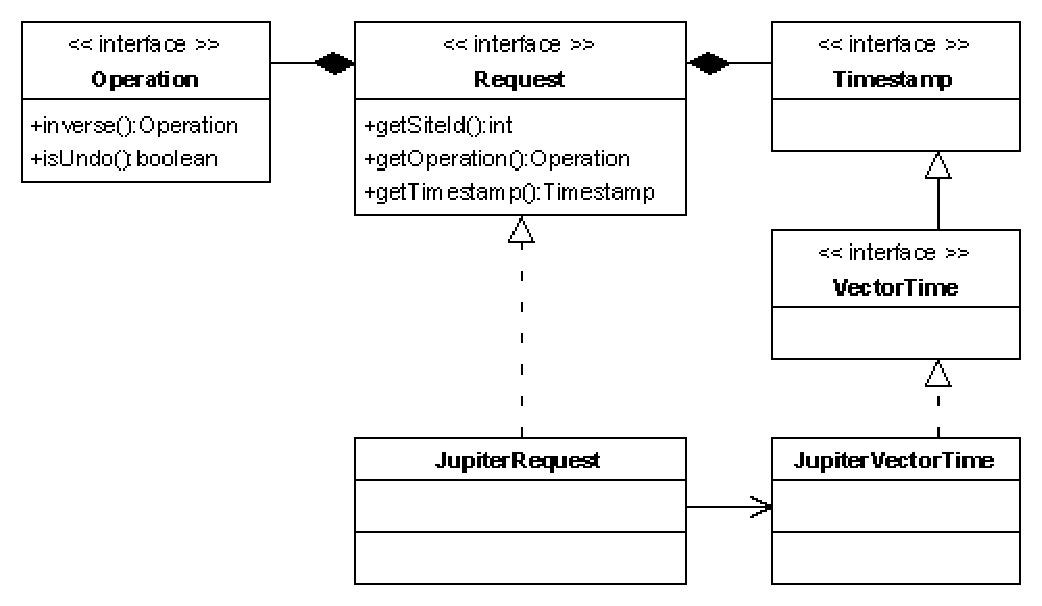
\includegraphics[height=6.87cm,width=12.09cm]{../images/finalreport/algorithm_request.eps}
\caption{Request Class Diagram}
\label{Request Class Diagram}
\end{figure}

How a request will be sent to a server or another client is not part of this chapter and depends on the network technology (see \emph{Report Evaluation Network}) used.


\subsection{Algorithm}

\begin{figure}[H]
\centering
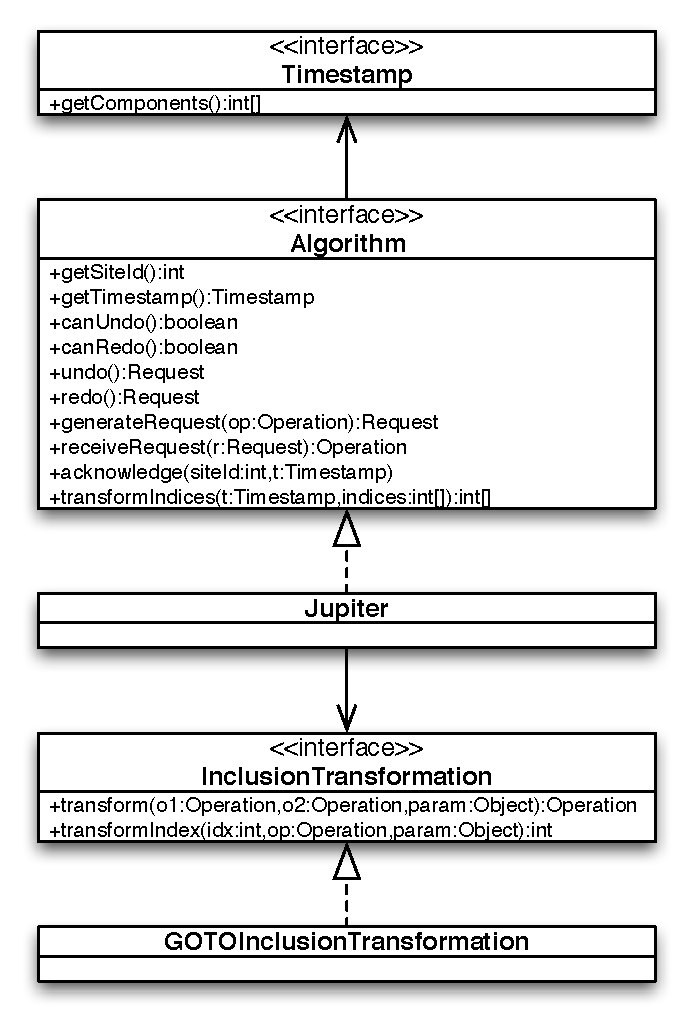
\includegraphics[height=12.09cm,width=6.87cm]{../images/finalreport/algorithm.eps}
\caption{Algorithm Class Diagram}
\label{fig:algorithm.uml}
\end{figure}

The algorithm package centers around the \texttt{Algorithm} interface.
It gives the flexibility to switch the implementation without affecting the 
rest of the system. The currently only implementation of the \texttt{Algorithm} 
interface is the \texttt{Jupiter} class. \texttt{Jupiter} processes 
all requests with the collaboration of an \texttt{InclusionTransformation}
implementation. The only implementation is \texttt{GOTOInclusionTransformation}.

Each algorithm has a local timestamp, which can be retrieved with the
\texttt{getTimestamp():Timestamp} method. In the 
case of \emph{Jupiter}, the timestamp is a vector time. The vector 
time represents the current location in the 2-dimensional state space of 
\emph{Jupiter}. 

The site id assigned to the algorithm can be retrieved with the
\texttt{getSiteId():int} method. The site id can be important in certain
transformation cases to decide which operation has higher priority, i.e.
is not shifted.

\subsubsection{Outgoing Queue}
\label{sect:algorithm.outgoingqueue}
\emph{Jupiter} stores all outgoing requests in a queue. Whenever a request
is received by the algorithm, the timestamp of the request is checked to
see how many requests the other site has already processed. All the requests
in the outgoing queue that have been processed by the other site are discarded.
The incoming request is then transformed against the the remaining requests
in the queue. The transformed operation is then ready to be applied to the
local document.

The figure \ref{fig:algorithm.outqueue} shows on the left side an outgoing
queue with four operations. Now, suppose a request with timestamp $[0,2]$
is received, indicating that the other site has processed two requests
from the local site. The first two requests in the queue can then be
discarded, leaving us with just two requests. The incoming request is then
transformed against these two (concurrent) requests.

\begin{figure}[H]
\centering
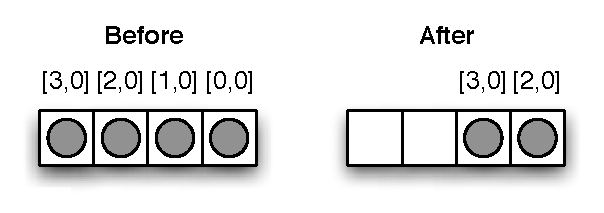
\includegraphics[height=3.03cm,width=9.67cm]{../images/finalreport/algorithm_outqueue.eps}
\caption{Outgoing queue before and after receiving a request}
\label{fig:algorithm.outqueue}
\end{figure}

\subsubsection{Generating Requests}
Whenever a local operation is generated it has to be sent to the other sites.
These operations must be encapsulated in a request. The
\texttt{generateRequest(op:Operation):Request} is used to create a request
for the operation. That request can be sent to the other sites.

\subsubsection{Receiving Requests}
When a request is received, it must be passed to the
\texttt{receiveRequest(r:Request):Operation} method. This method returns
the potentially transformed operation, which is to be applied to the
local document.

\subsubsection{Undo/Redo}
The \texttt{Algorithm} interface also has methods to support undo and redo.
The corresponding methods are \texttt{undo():Request}, \texttt{redo():Request},
\texttt{canUndo():boolean}, and \texttt{canRedo():boolean}. Unfortunately
\emph{Jupiter} does not support these operations. For more information why
\emph{Jupiter} does not support undo/redo read \ref{sect:algorithm.undoredo}.

\subsubsection{Index Transformations}
Beside the transformation of operations against other operations, the
\texttt{Algorithm} also supports transformation of an index against an
operation. 

The \texttt{transformIndices(t:Timestamp,indices:int[]):int[]} method transforms
an array of integers against all concurrent operations. The indices itself
do not modify the operations in the transformation.

\subsubsection{Acknowledge}
A potential problem arises if one site is idle while the other is generating
requests. In that case, the outgoing queue of the site that generates requests
grows indefinitely, because no acknowledge messages are ever received and thus
no requests in the outgoing queue are discarded.

Thus we extended the standard \emph{Jupiter} algorithm to support acknowledge
messages. An acknowledge message is simply the local timestamp and the site
id. An acknowledge message is passed to the algorithm with the
\texttt{acknowledge(siteId:int,t:Timestamp)} method.



